\subsection{Applicazione web}
La componente \textit{web-app} ha il compito di interfacciare gli utenti con i dispositivi visibili al loro ente di appartenenza, permettendo di visualizzare grafici contenenti i dati di determinati sensori o di modificare le configurazioni dei gateway stessi, aggiungendo o rimuovendo dispositivi e/o sensori. 

	\subsubsection{Diagrammi delle classi}
	Per semplificare il diagramma complessivo dell'applicazione web, le componenti model e controller sono state suddivise in due diagrammi separati.
	\begin{landscape}
		\begin{figure}[H]
			\centering
			\includegraphics[scale=0.600]{res/images/WEBAPP/ModelWebApp.png}
			\caption{Diagramma delle classi del model della componente web-app}
		\end{figure}
		\begin{figure}[H]
			\centering
			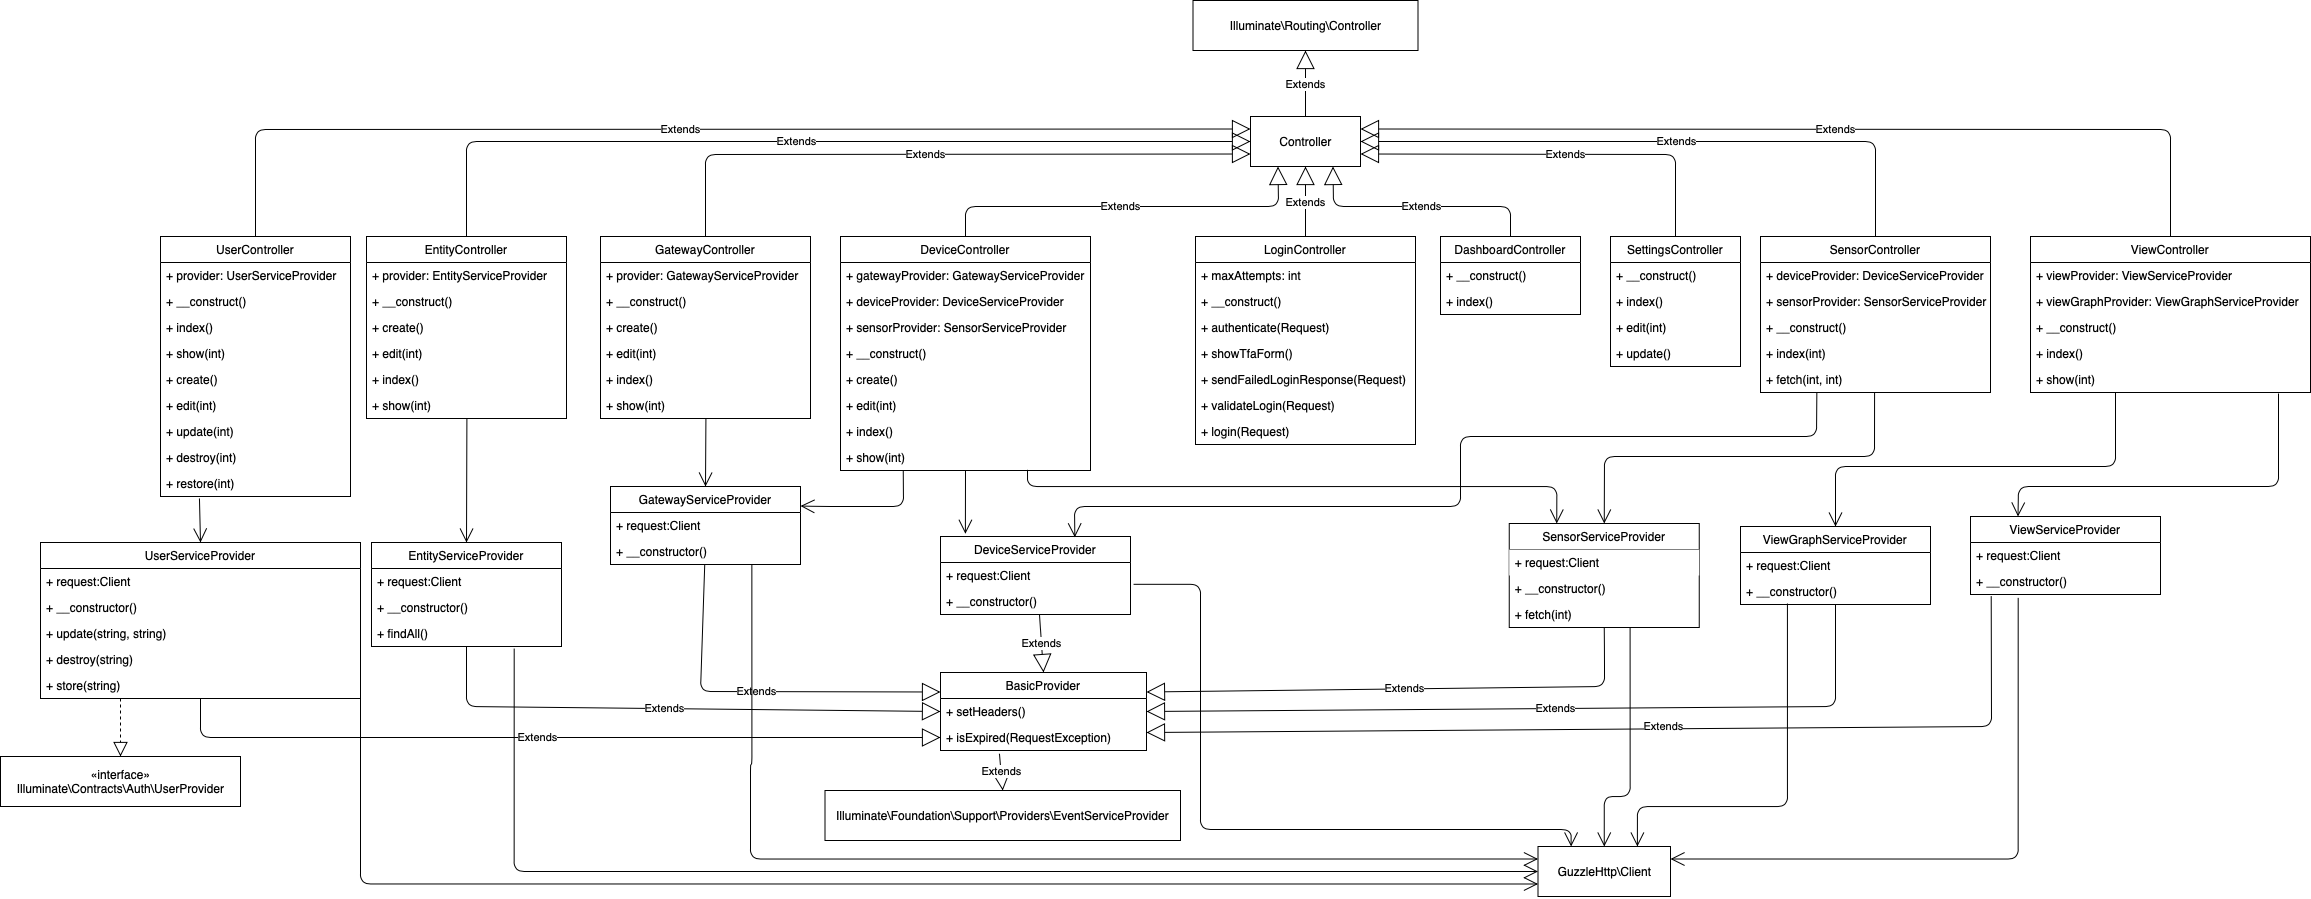
\includegraphics[scale=0.300]{res/images/WEBAPP/ControllerWebApp.png}
			\caption{Diagramma delle classi del controller della componente web-app}
		\end{figure}
		\end{landscape}
	\subsubsection{Diagrammi di sequenza}
	\subsubsection{Diagrammi di attività}